\documentclass[Master]{subfiles}
\begin{document}
\subsection{Majorana Fermions}
Ettore Majorana originally proposed the idea of Majorana particles as a purely real solution to the Dirac equation \cite{majorana1937teoria}. In solid state physics, Majorana fermions can occur as Bogoliubov quasi-particles. Any pair of fermionic creation and annihilation operators can be transformed to Majorana operators $\gamma_a$ and $\gamma_b$ with $\gamma_{a/b}^{\dag}=\gamma_{a/b}$ by :
$$
\frac{1}{\sqrt{2}} 
\underbrace{\left(\begin{array}{cc}
 1 & i \\
 1 & -i \\
\end{array}
\right)}_{U^{\dag}}
 \left(
\begin{array}{c}
 \gamma _{A,x} \\
 \gamma _{B,x} \\
\end{array}
\right)=\left(
\begin{array}{c}
 c_x \\
 c_x^{\dagger } \\
\end{array}
\right)
$$
$$
\frac{1}{\sqrt{2}} 
\underbrace{\left(
\begin{array}{cc}
 1 & 1 \\
 -i & i \\
\end{array}
\right)}_{U} \left(
\begin{array}{c}
 c_k \\
c_k^{\dagger } \\
\end{array}
\right)=\left(
\begin{array}{c}
 \gamma _{a,k} \\
 \gamma _{b,k} \\
\end{array}
\right)
$$
$$\gamma_{A}^2 = \gamma_{B}^2 = \mathbb{1}$$
Any fermion Hamiltonian can be written in majorana modes, but the eigenstates of the Hamiltonian are in general only fermionic see \secref{sec:Fermionicness}. However, when the ground state is a degenerate, the zero energy eigenstates span a subspace that contains some majorana modes. So the majorana modes can become eigenstates with eigenvalue zero as, when a degenerate ground state is present.
\subsubsection{Kitaev Model}\label{sec:KiteavModel}
A simple example where such zero energy majorana modes occur is the Kitaev Model \cite{kitaev2001unpaired}. 
\\
Given spin less fermions on a 1D chain with hopping term $t$, Chemical Potential $\mu$ and pair creation/annihilation term $\Delta$. The Hamiltonian becomes
\begin{dmath}\label{math:kitaevChainLat}
H = \sum_j - t (c^{\dag}_j c_{j+1}+c^{\dag}_{j+1} c_j) + \mu c^{\dag}_j c_j + |\Delta| (c^{\dag}_{j+1}c^{\dag}_j + c_j c_{j+1})
\end{dmath}
The lattice Hamiltonian can be Fourier transformed and written in Bogoliubov de Gennes form:
$$
H_{BdG} = \frac{1}{2}\sum_p (c_p^{\dag}, c_{-p})
\left( \begin{array}{cc}
    -2t \ cos \ p -\mu & 2|\Delta| i \ sin \ p  \\
     - 2 |\Delta| i \ sin \ p &  2t \ cos \ p +\mu
\end{array}\right)
\left(\begin{array}{c}
       c_p\\
       c_{-p}^{\dag}
\end{array}\right)
$$
The energy spectrum is 
$$
E(p) = \pm \sqrt{(2t \cos p + \mu)^2 + 4t |\Delta|^2\sin^2 p}
$$
This is called a p-wave superconductor, as the paring term is proportional to $p$ and vanishes for $p=0$.
The spectrum contains critical points for $|2t|>|\mu|: |\Delta|=0$ and $\mu = \pm 2 t : |\Delta|>0$.
The phases $|2t|<|\mu|: |\Delta|=0$ and $|2t|<|\mu|: |\Delta|>0$ are trivially connected. Thus, a topological phase can only exist $|\mu| < |2 t| : |\Delta|>0$. When we transform the Hamiltonian \eqref{math:kitaevChainLat} to Majorana modes the terms mix and give three new terms:
$$
H_{BdG} = \frac{i}{\sqrt{2}} \sum_j ( - \mu \gamma_{A,j}\gamma_{B,j} + (t + |\Delta|)\gamma_{B,j}\gamma_{A,j+1} +
(-t + |\Delta|)\gamma_{A,j}\gamma_{B,j+1}
)
$$
The three new terms can be visualised as in \figref{fig:Kitaevl} connecting different modes.
\begin{figure}[H]
    \centering
    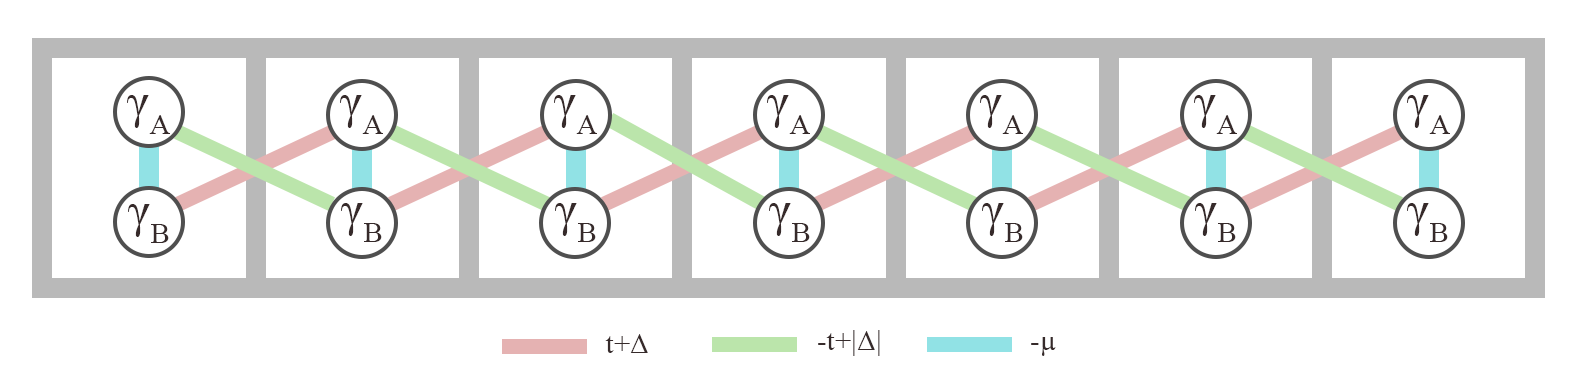
\includegraphics{imgs/Kitaev.png}
    \caption{Symbolic image of Kitaev Model for Majorana modes interactions of the three terms indicated as coloured lines}
    \label{fig:Kitaevl}
\end{figure}
For the special case $\mu = 0; |\Delta| = t >0$ Only the last term remains. compare to \figref{fig:Kitaev-top}
$$
H_{BdG} = \frac{i}{2} \sum_{j=0}^{N-1} ( 
-t + |\Delta|)\gamma_{A,j}\gamma_{B,j+1}
$$
\begin{figure}[H]
    \centering
    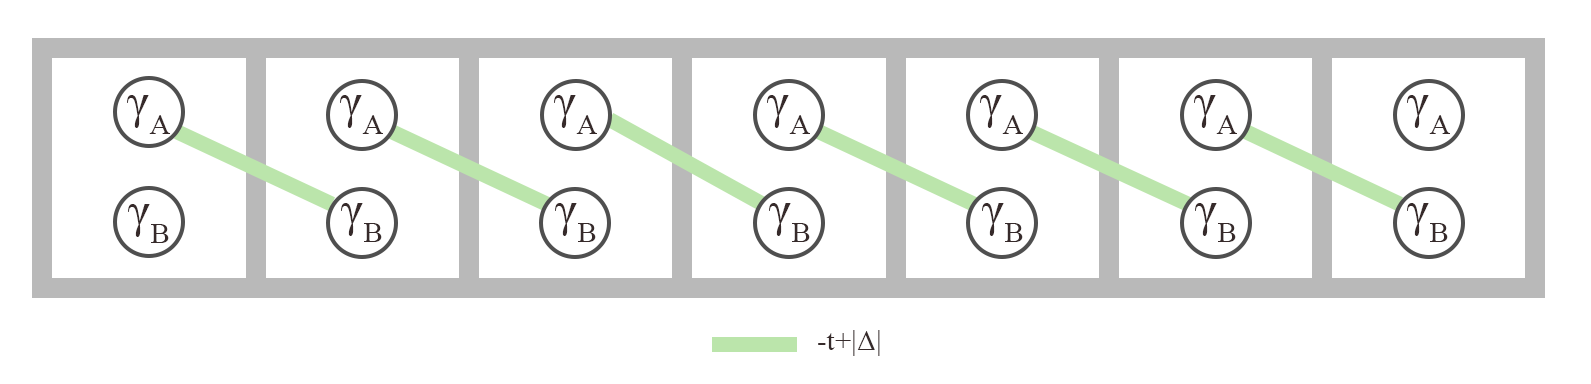
\includegraphics{imgs/Kitaev-top.png}
    \caption{Symbolic image of Kitaev model in the topological regime with free modes}
    \label{fig:Kitaev-top}
\end{figure}
Explicitly, in this special regime the Hamiltonian does not contain the operators $\gamma_{B,0}, \gamma_{A,N}$ Thus, there is a zero energy mode destroyed by  $c = \gamma_{A,N} + i \gamma_{B,0,}$ and created by $c^{\dag} = \gamma_{A,N} - i \gamma_{B,0,}$. The ground state is degenerate, and the majorana modes are eigenstates. The fermionic zero energy mode is delocalised as it acts on both ends of the chain, while the zero energy majorana modes are localised at one end of the chain.

These free Majorana modes are the edge modes predicted in \secref{sec:BulkEdgeCorrespondance}.
The corresponding topological phase lies in the $\mu < 2 t : |\Delta|>0$ region. A similar term exists for $\mu = 0; |\Delta| = - t > 0$ which is in the region $\mu > 2 t : |\Delta|>0$.

Topologically, the system has a induced charge conjugation symmetry $\mathcal{C} = \sigma^x K$, with $K$ the complex conjugation operator but no chiral $\mathcal{S}$ or time reversal symmetry $\mathcal{T}$ so it classifies as a topological D type. As it lives in 1D we expect a $\mathbb{Z}_2$ invariant. 
%There exist two equivalent ways to compute the topological invariant \cite{budich2013equivalent}.
%The derivation from Kitaev \cite{kitaev2001unpaired} rewrites the Majorana BdG Hamiltonian as a skew hermitian matrix
%$$H_{BdG} = \sum_{i,j} \gamma_i A_{i,j}\gamma_j$$
%The topological invariant is then $sign(Pf(A))$.
%The equivalent way is to compute the winding number over half the brillouin zone.
%Let $W(p) M(p) W^{\dag}(p) = D$ diagonalize the BdG Matrix:
%$$
%\Phi_{ZB} = i \int_0^{\pi} dp \ Tr[W^{\dag}(p)\partial_p W(p)]
%= i \int_0^{\pi} dp  \ \partial_p \log(\det(U W(p) U^{\dag})) 
%$$ 
%\begin{figure}[H]
%    \centering
%    \includegraphics{imgs/KitaevTopInvariant.png}
%    \caption{Topological Invariant of the Kitaev chain}
%    \label{fig:TopInvKiteav}
%\end{figure}
\end{document}